\section{Deployment Pipeline}

The deployment pipeline of the recommendation system involves setting up the Triton Ensemble and the external components of the system as shown in Figure \ref{fig:DeploymentDiagram}.

The steps involved in the deployment pipeline are as follows:

\subsubsection{Fetch User Features}

The Triton Ensemble fetches user features using the user ID, retrieving the necessary user-related data.

\subsubsection{Fetch Candidate Items}

The user features are processed by a TensorFlow retrieval model to generate a user embedding. This embedding is used to retrieve a list of candidate item IDs through a nearest neighbor search.

\subsubsection{Fetch Item Features}

The candidate item IDs are used to fetch item features.

\subsubsection{Unroll User Features}

User and item features are combined in the "Unroll User Features" step to prepare for scoring.

\subsubsection{Score Items}

The combined features are input into a TensorFlow scoring model, which predicts the relevance scores of each item.

\subsubsection{Order Items}

An ordering component uses these scores to rank the items, providing a list of recommendations as shown in Figure \ref{fig:ResponseList}.

\begin{figure}[H]
    \centering
    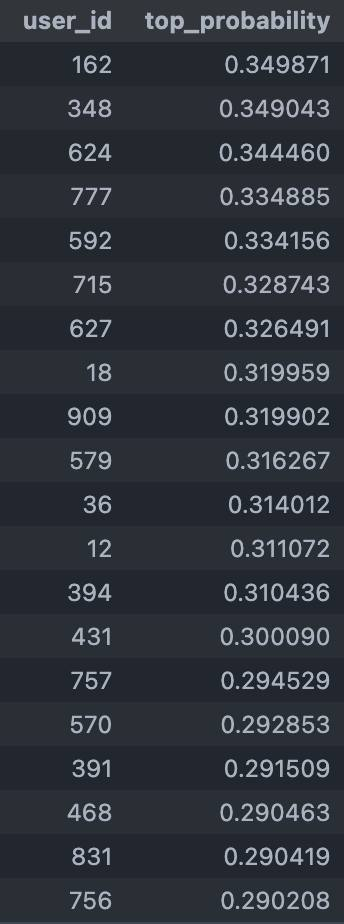
\includegraphics[width=0.4\textwidth]{assets/response_list.jpg}
    \caption{Response List}
    \label{fig:ResponseList}
\end{figure}


